\subsection{Ferramentas para engenharia de golems}

Portanto, se a tentativa de imitar a falsificação não é uma abordagem geralmente útil para os métodos estatísticos, o que devemos fazer? Devemos modelar. Modelos podem ser transformados em procedimentos de teste — todos os testes estatísticos também são modelos —, mas também podem ser usados para projetar, prever e argumentar. Fazer pesquisa se beneficia da capacidade de produzir e manipular modelos, tanto porque os problemas científicos são mais gerais do que "testar" quanto porque os golems pré-fabricados que você talvez tenha encontrado em cursos introdutórios de estatística são inadequados para muitos contextos de pesquisa. Você pode nem mesmo saber qual modelo estatístico usar, a menos que tenha um modelo generativo adicionalmente.

Se você quiser reduzir suas chances de destruir Praga, então é necessário algum \textit{know-how} de engenharia de golems. Não se engane: você destruirá Praga eventualmente. Mas se você for um bom engenheiro de golems, pelo menos notará a destruição. E como você saberá muito sobre como seu golem funciona, terá uma boa chance de descobrir o que deu errado. Então seu próximo golem não será tão ruim. Sem o treinamento em engenharia, você estará sempre à mercê de outra pessoa.

Queremos usar nossos modelos para vários propósitos distintos: projetar a investigação, extrair informações dos dados e fazer previsões. Neste livro, escolhi focar em ferramentas que ajudam em cada propósito. Essas ferramentas são:

\begin{enumerate}
  \item Análise de dados bayesiana
  \item Comparação de modelos
  \item Modelos multinível
  \item Modelos causais gráficos
\end{enumerate}

Essas ferramentas estão profundamente relacionadas umas com as outras, então faz sentido ensiná-las juntas. A compreensão dessas ferramentas vem, como sempre, apenas com a implementação — você não pode compreender a engenharia de golems até fazê-la. E por isso este livro se concentra principalmente no código, em como fazer as coisas. Mas no restante deste capítulo, forneço introduções a essas ferramentas.

\subsubsection{Análise de dados bayesiana}

Supondo que você tenha alguns dados, como deve usá-los para aprender sobre o mundo? Não há uma única resposta correta para essa pergunta. Muitas abordagens, tanto formais quanto heurísticas, podem ser eficazes. Mas uma das respostas mais eficazes e gerais é usar a análise de dados bayesiana. A análise de dados bayesiana pega uma pergunta na forma de um modelo e usa a lógica para produzir uma resposta na forma de distribuições de probabilidade.

Em termos modestos, a análise de dados bayesiana não é mais do que contar os números de maneiras que os dados poderiam acontecer, de acordo com nossas suposições. Coisas que podem acontecer de mais maneiras são mais plausíveis. A teoria das probabilidades é relevante porque a probabilidade é apenas um cálculo para contar. Isso nos permite usar a teoria das probabilidades como uma maneira geral de representar plausibilidade, seja em referência a eventos contáveis no mundo ou a construtos teóricos como parâmetros. O resto segue logicamente. Uma vez que definimos o modelo estatístico, a análise de dados bayesiana força uma maneira puramente lógica de processar os dados para produzir inferência.

O Capítulo 2 explica isso em profundidade. Por enquanto, ajudará ter outra abordagem para comparar. A probabilidade bayesiana é uma abordagem muito geral da probabilidade e inclui, como um caso especial, outra abordagem importante, a abordagem \textsc{frequentista}. A abordagem frequentista exige que todas as probabilidades sejam definidas por meio da conexão com as frequências de eventos em amostras muito grandes. Isso leva a incerteza frequentista a ser baseada em uma reamostragem imaginária de dados — se fôssemos repetir a medição muitas e muitas vezes, acabaríamos coletando uma lista de valores que teria algum padrão. Significa também que parâmetros e modelos não podem ter distribuições de probabilidade, apenas as medições podem. A distribuição dessas medições é chamada de \textsc{distribuição amostral}. Essa reamostragem nunca é feita e, em geral, nem faz sentido — é absurdo considerar a reamostragem repetida da diversificação de pássaros canoros nos Andes. Como Sir Ronald Fisher, um dos estatísticos frequentistas mais importantes do século XX, colocou:

\begin{quote}
  [...] as únicas populações que podem ser referidas em um teste de significância não têm realidade objetiva, sendo exclusivamente produto da imaginação do estatístico [...]
\end{quote}

Mas em muitos contextos, como em experimentos controlados em estufas, é um dispositivo útil para descrever a incerteza. Qualquer que seja o contexto, é apenas parte do modelo, uma suposição sobre como os dados seriam sob reamostragem. É tão fantástico quanto a aposta bayesiana de usar a probabilidade para descrever todos os tipos de incerteza, sejam empíricas ou epistemológicas.

Mas essas diferentes atitudes em relação à probabilidade impõem \textit{trade-offs} diferentes. Considere este exemplo simples onde a diferença entre probabilidade bayesiana e frequentista importa. No ano de 1610, Galileu apontou um telescópio primitivo para o céu noturno e se tornou o primeiro ser humano a ver os anéis de Saturno. Bem, ele provavelmente viu um borrão, com alguns borrões menores presos a ele (FIGURA 1.3). Como o telescópio era primitivo, ele realmente não conseguia focar muito bem a imagem. Saturno sempre parecia desfocado. Este é um problema estatístico, de certa forma. Há incerteza sobre a forma do planeta, mas observe que nenhuma incerteza é resultado de variação em medições repetidas. Poderíamos olhar pelo telescópio mil vezes, e ele sempre daria a mesma imagem desfocada (para qualquer posição dada da Terra e de Saturno). Portanto, a distribuição amostral de qualquer medição é constante, porque a medição é determinística — não há nada "aleatório" nisso. A inferência estatística frequentista tem muitos problemas para começar aqui. Em contraste, a inferência bayesiana prossegue como de costume, porque o "ruído" determinístico ainda pode ser modelado usando a probabilidade, desde que não identifiquemos probabilidade com frequência. Como resultado, o campo de reconstrução e processamento de imagens é dominado por algoritmos bayesianos.

% INSERIR A FIGURA 1.3 AQUI
\begin{figure}[htbp]
  \centering
  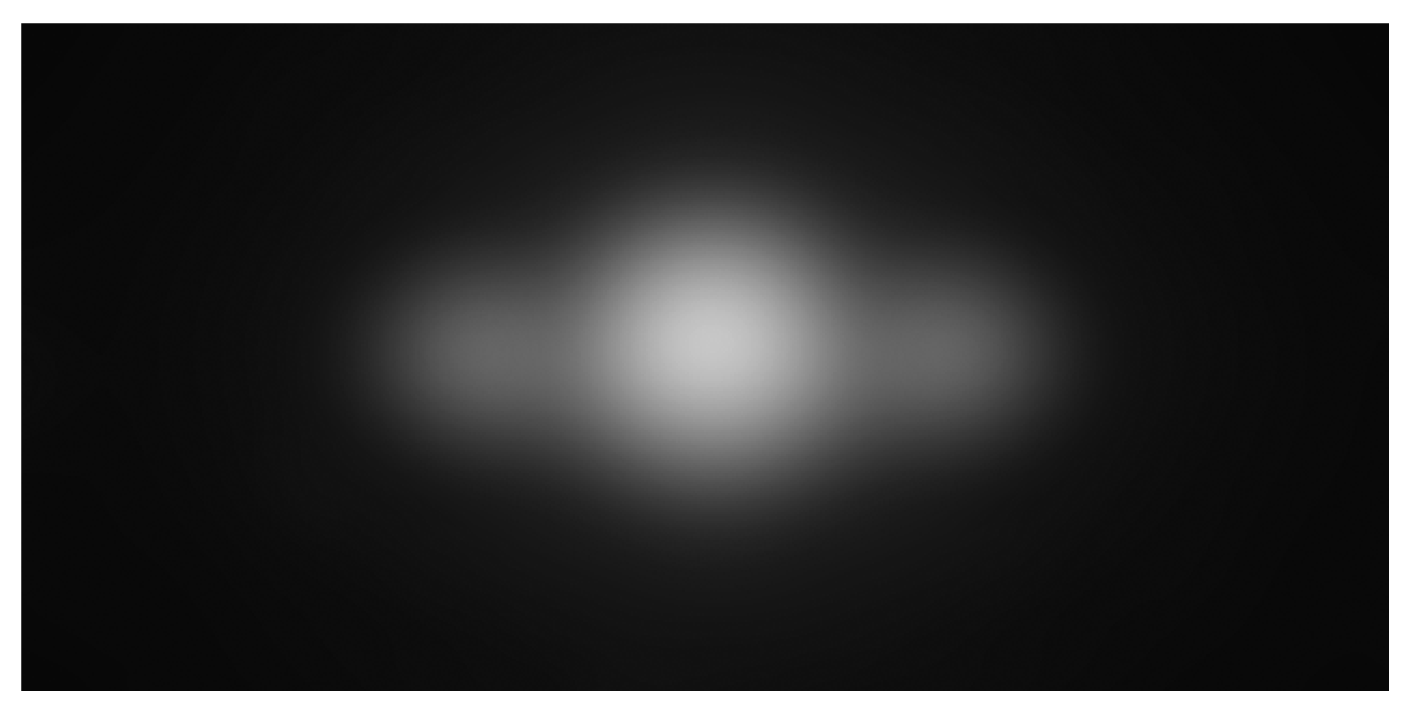
\includegraphics[width=\textwidth]{img/fig1_3.png}
  \caption{Saturno, muito parecido com o que Galileu deve ter visto. A forma verdadeira é incerta, mas não por causa de qualquer variação de amostragem. A teoria das probabilidades ainda pode ajudar.}
  \label{fig:1.3}
\end{figure}

Em procedimentos estatísticos mais rotineiros, como a regressão linear, essa diferença nos conceitos de probabilidade tem menos efeito. No entanto, é importante perceber que, mesmo quando um procedimento bayesiano e um procedimento frequentista dão exatamente a mesma resposta, nossos golems bayesianos não estão justificando suas inferências com reamostragens repetidas imaginadas. De forma mais geral, os golems bayesianos tratam a "aleatoriedade" como uma propriedade da informação, não do mundo. Nada no mundo real — exceto interpretações controversas da física quântica — é realmente aleatório. Presumivelmente, se tivéssemos mais informações, poderíamos prever tudo exatamente. Nós apenas usamos a aleatoriedade para descrever nossa incerteza diante do conhecimento incompleto. Da perspectiva do nosso golem, o lançamento da moeda é "aleatório", mas na verdade é o golem que é aleatório, não a moeda.

Note que a descrição anterior não invoca as "crenças" ou opiniões subjetivas de ninguém. A análise de dados bayesiana é apenas um procedimento lógico para processamento de informações. Existe uma tradição de usar esse procedimento como uma descrição normativa da crença racional, uma tradição chamada \textsc{bayesianismo}. Mas este livro nem a descreve nem a defende. De fato, argumentarei que nenhuma abordagem estatística, bayesiana ou de outra forma, é por si só suficiente.

\begin{quote}
  \textbf{Repensando: A probabilidade não é unitária.} Deixará alguns leitores desconfortáveis sugerir que há mais de uma maneira de definir "probabilidade". Os conceitos matemáticos não são unicamente corretos? Eles não são. Depois de adotar algum conjunto de premissas, ou axiomas, tudo se segue logicamente em sistemas matemáticos. Mas os axiomas estão abertos ao debate e à interpretação. Portanto, não existe apenas a probabilidade "bayesiana" e a "frequentista", mas também existem diferentes versões da probabilidade bayesiana, baseando-se em diferentes argumentos para justificar a abordagem. Em textos bayesianos mais avançados, você encontrará nomes como Bruno de Finetti, Richard T. Cox e Leonard "Jimmie" Savage. Cada uma dessas figuras está associada a uma concepção um tanto diferente da probabilidade bayesiana. Existem outras. Este livro segue principalmente a interpretação "lógica" de Cox (ou Laplace-Jeffreys-Cox-Jaynes). Esta interpretação é apresentada a partir do próximo capítulo, mas se desdobra totalmente apenas no Capítulo 10.

  Como podem prosperar diferentes interpretações da teoria das probabilidades? Por si mesmas, as entidades matemáticas não "significam" necessariamente nada, no sentido de implicação no mundo real. O que significa tirar a raiz quadrada de um número negativo? O que significa tirar um limite quando algo se aproxima do infinito? Esses são conceitos essenciais e rotineiros, mas seus significados dependem do contexto e do analista, das crenças sobre o quão bem a abstração representa a realidade. A matemática não acessa o mundo real diretamente. Portanto, responder a tais perguntas continua sendo um projeto contencioso e divertido, em todos os ramos da matemática aplicada. Portanto, embora todos subscrevam os mesmos axiomas de probabilidade, nem todos concordam em todos os contextos sobre como interpretar a probabilidade.
\end{quote}

Antes de passar a descrever as próximas duas ferramentas, vale a pena enfatizar uma vantagem da análise de dados bayesiana, pelo menos quando estudiosos estão aprendendo modelagem estatística. Este livro inteiro poderia ser reescrito para remover qualquer menção ao termo "bayesiano". Em alguns lugares, ficaria mais fácil. Em outros, ficaria muito mais difícil. Mas, tendo ensinado estatística aplicada das duas maneiras, descobri que a estrutura bayesiana apresenta uma vantagem pedagógica distinta: muitas pessoas a acham mais intuitiva. Talvez a melhor evidência disso seja que muitos cientistas interpretam resultados não bayesianos em termos bayesianos, por exemplo, interpretando valores-$p$ ordinários como probabilidades bayesianas \textit{a posteriori} e intervalos de confiança não bayesianos como intervalos bayesianos (você aprenderá sobre probabilidade \textit{a posteriori} e intervalos de confiança nos Capítulos 2 e 3). Até mesmo instrutores de estatística cometem esses erros. Neste sentido, então, os modelos bayesianos levam a interpretações mais intuitivas, aquelas que os cientistas tendem a projetar em resultados estatísticos. O padrão oposto de erro — interpretar uma probabilidade \textit{a posteriori} como um valor-$p$ — parece acontecer apenas raramente.

Nada disso garante que as análises bayesianas serão mais corretas do que as análises não bayesianas. Significa apenas que as intuições do cientista estarão menos comumente em desacordo com a lógica real da estrutura. Isso simplifica alguns dos aspectos do ensino da modelagem estatística.

\begin{quote}
  \textbf{Repensando: Um pouco de história.} A inferência estatística bayesiana é muito mais antiga do que as ferramentas típicas da estatística introdutória, a maioria das quais foi desenvolvida no início do século XX. Versões da abordagem bayesiana foram aplicadas ao trabalho científico no final dos anos 1700 e repetidamente no século XIX. Mas, após a Primeira Guerra Mundial, estatísticos antibayesianos, como Sir Ronald Fisher, conseguiram marginalizar a abordagem. Tudo o que Fisher disse sobre a análise bayesiana (então chamada de \textit{probabilidade inversa}) em seu influente manual de 1925 foi:

  \begin{quote}
    [...] a teoria da probabilidade inversa baseia-se num erro e deve ser totalmente rejeitada.
  \end{quote}

  A análise de dados bayesiana tornou-se cada vez mais aceita dentro da estatística durante a segunda metade do século XX, porque provou não ser baseada em um erro. Deixando toda filosofia de lado, ela funcionava. Começando na década de 1990, novas abordagens computacionais levaram a um rápido aumento na aplicação de métodos bayesianos. Os métodos bayesianos permanecem computacionalmente caros, no entanto. E, à medida que os conjuntos de dados aumentaram de escala — milhões de linhas é comum na análise genômica, por exemplo —, alternativas ou aproximações à inferência bayesiana permanecem importantes e provavelmente sempre o serão.
\end{quote}

\subsubsection{Comparação de modelos e previsão}

A análise de dados bayesiana fornece uma maneira para os modelos aprenderem com os dados. Mas quando há mais de um modelo plausível — e na maioria dos campos maduros deveria haver —, como devemos escolher entre eles? Uma resposta é preferir modelos que façam boas previsões. Essa resposta cria muitas perguntas novas, já que saber qual modelo fará as melhores previsões parece exigir conhecer o futuro. Analisaremos profundamente duas ferramentas relacionadas, nenhuma das quais conhece o futuro: \textsc{validação cruzada} e \textsc{critérios de informação}. Essas ferramentas visam nos permitir comparar modelos com base na precisão preditiva esperada.

Comparar modelos pela precisão preditiva pode ser útil por si só. E será ainda mais útil porque leva à descoberta de um fato surpreendente: modelos complexos muitas vezes fazem previsões piores do que modelos mais simples. O paradoxo primário da previsão é o \textsc{overfitting}: \textit{O ajuste é fácil; a previsão é difícil.} Dados futuros não serão exatamente iguais aos dados passados e, portanto, qualquer modelo que não esteja ciente desse fato tende a fazer previsões piores do que poderia. E modelos mais complexos tendem a sofrer mais \textsc{overfitting} do que os simples — quanto mais inteligente o golem, mais burras suas previsões. Portanto, se desejamos fazer boas previsões, não podemos julgar nossos modelos simplesmente pelo quão bem eles se ajustam aos nossos dados.

A validação cruzada e os critérios de informação nos ajudam de três maneiras relacionadas. Primeiro, eles fornecem expectativas úteis de precisão preditiva, em vez de um mero ajuste à amostra. Assim, eles comparam modelos onde isso importa. Segundo, eles nos dão uma estimativa da tendência de um modelo de sofrer \textsc{overfitting} nos dados. Isso nos ajudará a entender como modelos e dados interagem, o que, por sua vez, nos ajuda a projetar modelos melhores. Retomaremos esse ponto na próxima seção. Terceiro, a validação cruzada e os critérios de informação podem nos ajudar a identificar observações altamente influentes.

A análise de dados bayesiana vem sendo trabalhada há séculos. Os critérios de informação são comparativamente muito jovens e o campo está evoluindo rapidamente. Muitos estatísticos nunca usaram critérios de informação em um problema aplicado, e não há consenso sobre quais métricas são as melhores e como melhor usá-las. Ainda assim, os critérios de informação já são de uso frequente nas ciências, aparecendo em publicações proeminentes e figurando em debates importantes. O poder deles é frequentemente exagerado, e teremos o cuidado de notar o que eles não podem fazer, bem como o que podem.

\begin{quote}
  \textbf{Repensando: O neandertal em você.} Até mesmo modelos simples precisam de alternativas. Em 2010, o rascunho de um genoma de um Neandertal demonstrou mais sequências de DNA em comum com humanos contemporâneos não africanos do que com africanos. Essa descoberta é consistente com o cruzamento entre neandertais e humanos modernos, à medida que os últimos se dispersaram da África. No entanto, apenas encontrar DNA em comum entre europeus modernos e neandertais não é suficiente para demonstrar o cruzamento. Também é consistente com a estrutura antiga no continente africano. Em suma, se os antigos nordestinos da África tivessem sequências de DNA únicas, então neandertais e europeus modernos poderiam possuir essas sequências de um ancestral comum, em vez de por cruzamento direto. Portanto, mesmo no caso aparentemente simples de estimar se neandertais e humanos modernos compartilham DNA único, há mais de uma explicação baseada em processo. A comparação de modelos é necessária.
\end{quote}

\subsubsection{Modelos multinível}

Em um conto apócrifo da cosmologia hindu, diz-se que a Terra repousa nas costas de um grande elefante, que por sua vez fica nas costas de uma enorme tartaruga. Quando perguntado sobre o que a tartaruga está apoiada, diz-se que um guru responde: "é tartaruga até lá embaixo."

Modelos estatísticos não contêm tartarugas, mas eles contêm parâmetros. E os parâmetros sustentam a inferência. Sobre o que os próprios parâmetros se apoiam? Às vezes, em alguns dos modelos mais poderosos, são parâmetros até lá embaixo. O que isso significa é que qualquer parâmetro particular pode ser proveitosamente considerado como um marcador de posição para um modelo ausente. Dado algum modelo de como o parâmetro obtém seu valor, é bastante simples incorporar o novo modelo dentro do antigo. Isso resulta em um modelo com múltiplos níveis de incerteza, cada um alimentando o próximo — um \textsc{modelo multinível}.

Modelos multinível — também conhecidos como modelos hierárquicos, de efeitos aleatórios, de efeitos variados ou de efeitos mistos — estão se tornando \textit{de rigueur} nas ciências biológicas e sociais. Campos tão diversos quanto testes educacionais e filogenética bacteriana agora dependem de modelos multinível rotineiros para processar dados. Assim como a análise de dados bayesiana, a modelagem multinível não é particularmente nova, mas ela está disponível em computadores pessoais há apenas algumas décadas. E como tais modelos têm uma representação bayesiana natural, eles cresceram lado a lado com a análise de dados bayesiana.

Estaremos interessados em modelos multinível principalmente porque eles nos ajudam a lidar com o \textsc{overfitting}. A validação cruzada e os critérios de informação medem o risco de \textsc{overfitting} e nos ajudam a reconhecê-lo. Mas os modelos multinível realmente fazem algo a respeito. O que eles fazem é explorar um truque estatístico incrível conhecido como \textsc{agrupamento parcial} (\textit{partial pooling}) que agrupa informações entre as unidades nos dados para produzir estimativas melhores para todas as unidades. Os detalhes aguardarão até o Capítulo 13.

O agrupamento parcial é a tecnologia-chave, e os contextos nos quais ele é apropriado são diversos. Aqui estão quatro exemplos comuns.

\begin{enumerate}
  \item \textit{Para ajustar as estimativas para amostragem repetida.} Quando mais de uma observação surge do mesmo indivíduo, local ou época, então os modelos tradicionais de nível único podem nos enganar.
  \item \textit{Para ajustar as estimativas para desequilíbrio na amostragem.} Quando alguns indivíduos, locais ou épocas são amostrados mais do que outros, também podemos ser enganados por modelos de nível único.
  \item \textit{Para estudar a variação.} Se nossas questões de pesquisa incluem a variação entre indivíduos ou outros grupos dentro dos dados, então os modelos multinível são uma grande ajuda, porque eles modelam a variação explicitamente.
  \item \textit{Para evitar tirar médias.} Frequentemente, os pesquisadores tiram a média de alguns dados antecipadamente para construir variáveis para uma análise de regressão. Isso pode ser perigoso, porque a média remove a variação. Portanto, fabrica-se uma falsa confiança. Os modelos multinível nos permitem preservar a incerteza nos valores originais, anteriores à média, e ainda assim usar a média para fazer previsões.
\end{enumerate}

Todos os quatro se aplicam a contextos nos quais o pesquisador reconhece \textit{clusters} ou grupos de medições que podem diferir uns dos outros. Esses \textit{clusters} ou grupos podem ser indivíduos como alunos diferentes, locais como cidades diferentes ou períodos como anos diferentes. Como cada \textit{cluster} pode muito bem ter uma tendência média diferente ou responder de maneira diferente a qualquer tratamento, os dados agrupados frequentemente se beneficiam de serem modelados por um golem que espera essa variação.

Mas o escopo da modelagem multinível é muito maior do que esses exemplos. Diversos tipos de modelos acabam sendo multinível: modelos para dados ausentes (imputação), erro de medição, análise fatorial, alguns modelos de séries temporais, tipos de regressão espacial e de rede e regressões filogenéticas são todos aplicações especiais da estratégia multinível. Compreender o conceito de modelagem multinível pode levar a uma mudança de perspectiva. De repente, modelos de nível único acabam parecendo meros componentes de modelos multinível. A estratégia multinível fornece um princípio de engenharia para nos ajudar a introduzir esses componentes em uma análise particular, exatamente onde achamos que precisamos deles.

Quero convencer o leitor de algo que parece irracional: \textit{a regressão multinível merece ser a forma padrão de regressão}. Trabalhos que não usam modelos multinível deveriam justificar o fato de não usarem uma abordagem multinível. Certamente, alguns dados e contextos não precisam do tratamento multinível. Mas a maioria dos estudos contemporâneos nas ciências sociais e naturais, sejam experimentais ou não, se beneficiaria disso. Talvez o motivo mais importante seja que mesmo os tratamentos bem controlados interagem com aspectos não medidos dos indivíduos, grupos ou populações estudadas. Isso leva a uma variação nos efeitos do tratamento, na qual indivíduos ou grupos variam na forma como respondem à mesma circunstância. Modelos multinível tentam quantificar a extensão dessa variação, bem como identificar quais unidades nos dados responderam de quais maneiras.

Esses benefícios não vêm de graça, no entanto. Ajustar e interpretar modelos multinível pode ser consideravelmente mais difícil do que ajustar e interpretar um modelo de regressão tradicional. Na prática, muitos pesquisadores simplesmente confiam em seus softwares de caixa-preta e interpretam a regressão multinível exatamente como a regressão de nível único. Com o tempo, isso vai mudar. Houve um tempo na estatística aplicada em que mesmo a regressão múltipla comum era considerada de ponta, algo apenas para especialistas mexerem. Em vez disso, os cientistas usavam muitos procedimentos simples, como testes $t$. Agora, quase todo mundo usa ferramentas multivariadas. O mesmo acabará sendo verdade para os modelos multinível. A cultura acadêmica e o currículo ainda têm algum atraso a recuperar.

\begin{quote}
  \textbf{Repensando: Previsão eleitoral multinível.} Uma das aplicações mais antigas da modelagem multinível é a previsão dos resultados das eleições democráticas. No início dos anos 1960, John Tukey (1915–2000) começou a trabalhar para a \textit{National Broadcasting Company} (NBC) nos Estados Unidos, desenvolvendo modelos de previsão de eleições em tempo real que poderiam explorar diversos tipos de dados: pesquisas, eleições passadas, resultados parciais e resultados completos de distritos relacionados. Os modelos usavam uma estrutura multinível semelhante aos modelos apresentados nos Capítulos 13 e 14. Tukey desenvolveu e usou esses modelos para a NBC até 1978. A previsão eleitoral contemporânea e a agregação de pesquisas continuam sendo um tópico ativo para modelagem multinível.
\end{quote}

\subsubsection{Modelos causais gráficos}

Quando o vento sopra, os galhos balançam. Se você é humano, imediatamente interpreta essa afirmação como causal: O vento faz os galhos se moverem. Mas tudo o que vemos é uma associação estatística. Apenas pelos dados, também poderia ser que o balançar dos galhos fizesse o vento. Essa conclusão parece tola, porque você sabe que as árvores não balançam seus próprios galhos. Um modelo estatístico é um incrível mecanismo de associação. Ele torna possível detectar associações entre causas e seus efeitos. Mas um modelo estatístico nunca é suficiente para inferir a causa, porque o modelo estatístico não faz distinção entre o vento fazer os galhos balançarem e os galhos fazerem o vento soprar. Fatos fora dos dados são necessários para decidir qual explicação está correta.

A validação cruzada e os critérios de informação tentam adivinhar a precisão preditiva. Quando os apresentei acima, descrevi o \textsc{overfitting} como o paradoxo primário da previsão. Agora nos voltamos para um paradoxo secundário da previsão: \textit{Modelos que são causalmente incorretos podem fazer previsões melhores do que aqueles que são causalmente corretos.} Como resultado, focar na previsão pode nos enganar sistematicamente. E embora você possa ter ouvido que experimentos controlados randomizados permitem a inferência causal, esses riscos também envolvem experimentos randomizados. Ninguém está seguro.

Chamarei a isso de problema de \textsc{identificação} e o distinguirei cuidadosamente do problema da previsão bruta. Considere dois significados diferentes de "previsão". O mais simples se aplica quando somos observadores externos simplesmente tentando adivinhar o que acontecerá a seguir. Nesse caso, ferramentas como a validação cruzada são muito úteis. Mas essas ferramentas recomendarão alegremente modelos que contêm variáveis de confusão e sugerem relações causais incorretas. Por quê? Relações confundidas são associações reais e podem melhorar a previsão. Afinal, se você olhar para fora e ver galhos balançando, isso realmente prediz o vento. O sucesso da previsão não requer a identificação causal correta. De fato, como você verá mais adiante no livro, as previsões podem realmente melhorar quando usamos um modelo que é causalmente enganoso.

Mas o que acontece quando intervimos no mundo? Agora tudo muda. Agora devemos considerar um segundo significado de "previsão": O que acontecerá quando intervirmos no mundo. Suponha que recrutemos muitas pessoas para subir nas árvores e balançar os galhos. Isso fará vento? Não muito. Muitas vezes, o ponto da modelagem estatística é produzir um entendimento que leve à generalização e aplicação. Nesse caso, precisamos de mais do que apenas boas previsões, na ausência de intervenção. Nós também precisamos de uma compreensão causal precisa. Mas comparar modelos com base na precisão preditiva — ou valores-$p$ ou qualquer outra coisa — não a produzirá necessariamente.

Então o que pode ser feito? O que é necessário é um modelo causal que possa ser usado para projetar um ou mais modelos estatísticos com o propósito de identificação causal. Como mencionei no exemplo de evolução molecular neutra mais cedo neste capítulo, um modelo científico completo contém mais informações do que um modelo estatístico derivado dele. E essa informação adicional contém implicações causais. A maioria dos cientistas faz uso informal dessas implicações. Mas também é possível fazer uso formal delas, demonstrando logicamente quando uma estimativa identifica uma relação causal. Esses métodos formais datam da primeira metade do século XX, mas eles foram estendidos mais recentemente ao estudo da medição, do desenho experimental e da capacidade de generalizar (ou \textit{transportar}) resultados entre as amostras.

E a excelente notícia é que mesmo quando você não tem um modelo causal completo, mas apenas um heurístico indicando quais variáveis influenciam causalmente outras, você ainda pode fazer uso dessas ferramentas lógicas. Essa é a estratégia que usaremos neste livro. Usaremos um \textsc{modelo causal gráfico} para representar uma hipótese causal. O modelo causal gráfico mais simples é um \textsc{grafo acíclico direcionado}, geralmente chamado de \textsc{DAG}. Os DAGs são heurísticos — eles não são modelos estatísticos detalhados. Mas eles nos permitem deduzir quais modelos estatísticos podem fornecer inferências causais válidas, assumindo que o DAG seja verdadeiro. Você não precisa entender isso agora. Os capítulos posteriores constroem DAGs por meio de exemplos.

Mas de onde vem o próprio DAG? A terrível verdade sobre a inferência estatística é que sua validade depende de informações fora dos dados. Nós requeremos um modelo causal com o qual projetar tanto a coleta de dados quanto a estrutura de nossos modelos estatísticos. Mas a construção de modelos causais não é um esforço puramente estatístico, e a análise estatística nunca pode verificar todas as nossas suposições. Nunca haverá um golem que aceite dados nus e retorne um modelo confiável das relações causais entre as variáveis. Teremos apenas que continuar fazendo ciência.

\begin{quote}
  \textbf{Repensando: Salada causal.} A inferência causal requer um modelo causal que seja separado do modelo estatístico. Os dados não são suficientes. Toda filosofia concorda quanto a isso. As respostas, no entanto, são diversas. A resposta mais conservadora é declarar a "causação" como um doce mental improvável, como debater a natureza da vida após a morte. Um pouco menos conservador é insistir que a causa só pode ser inferida sob condições estritas de randomização e controle experimental. Isso seria muito limitante. Muitas questões científicas nunca podem ser estudadas experimentalmente — a evolução humana, por exemplo. Muitas outras poderiam, em princípio, ser estudadas experimentalmente, mas seria antiético fazê-lo. E muitos experimentos são na verdade apenas tentativas de controle — pacientes nem sempre tomam sua medicação.

  Mas a abordagem que domina em muitas partes da biologia e das ciências sociais é, em vez disso, a \textsc{salada causal}. Salada causal significa jogar várias variáveis de "controle" em um modelo estatístico, observar mudanças nas estimativas e, em seguida, contar uma história sobre a causalidade. A salada causal parece fundada na noção de que apenas variáveis omitidas podem nos induzir em erro sobre a causação. Mas variáveis \textit{incluídas} podem nos confundir com a mesma facilidade. Ao misturar uma salada causal, um modelo que faz boas previsões ainda pode enganar sobre a causação. Se usarmos o modelo para planejar uma intervenção, ele errará tudo. Haverá exemplos em capítulos posteriores.
\end{quote}